\chapter{NDVI-MAP FUNCTIONS AND USER GUIDE}
\label{chap:tibet}

\section{What can app do?}

Handling \acrfull{ims} data at several resolutions requires significant data management efforts. Universal tasks include: Parsing through dates, filtering latitude and longitude coordinates, calculating snow/ice areas, and other functions that characterize \acrfull{sacd}. Individual groups who use IMS data dedicate time and resources developing and maintaining code built to handle these tasks. Currently, there is no \acrfull{foss} available for users. Consequentially groups and users are developing personal libraries to handle data, where they probably should be analyzing and drawing inferences from that data. In response to this challenge, a convenient toolkit for the snow-SACD has been created, with the \acrfull{tp} used as an example of the toolkit's capabilities.
The TP region, bounded by (25,45)$^\circ$N and (65,105)$^\circ$E, also known as the Third Pole of the Earth and includes the Himalaya Mountains, is used as an example to describe the 
SACD's method and usage.
TP region's average altitude is over 4000 meters. TP's snow cover area has a large annual cycle and a considerable temporal variation due to TP's strong interaction with the atmospheric flows during the Indian and the East Asian monsoons in the summer, as well as the westerlies from the Eurasian continent in the winter.  These interactions significantly affect the Earth surface's heat exchange with the atmosphere and can then influence the climate of southern and eastern Asia, even the global climate \cite{yao2012different, yao2013review}. 
Thus, TP’s snow cover has a notable influence on its regional and global climate. Its accurate monitoring is essential for understanding the climate variations of both TP and the world. Furthermore, accurate snow-cover information that the IMS data provides is critical for weather prediction and hydro-logical resource management efforts. In one example, Peings and Douville [2010] correlated the Indian monsoon and Eurasian Snowfall. They used 0.5◦ resolution satellite data over a long timescale. A finer resolution product such as the IMS can be used to re-evaluate their findings. Another study by Wu and Qian [2003] provided evidence for positive correlations between Tibetan snow and the East Asian Monsoon. They considered not only snow-covered area but also the snow depth from the field measurements of 60 Tibetan stations. The high-resolution IMS data can help more accurately quantify their results of snow cover. Although Shen et al. [2015] described the spatiotemporal variation of the TP snow cover using the IMS data, their results displayed in map projection percentage coverage. They did not provide a quantitative snow-cover area calculation in square kilometers and did not explore the actual TP surface area of each grid box in the polar stereographic projection. The nominal 24 km resolution on the projection plane needs to find its corresponding Earth surface grid boxes and their associated areas. The SACD toolkit described in this thesis is designed to solve this problem by providing each grid box’s surface area as shown in Figures~\ref{fig:areas_row_col} and \ref{fig:areas_tibet}. It can display IMS data with maps, and with a geographic background, and hence enriches the IMS’s software suites. Thus, the toolkit is useful for further study of snow cover, snow depth-snow water equivalence, climate forecast, and hydrological engineering planning and management. The SACD toolkit can map any region on the northern hemisphere
In addition to this thesis, the website \href{http://www.itsonlyamodel.us}({www.itsonlyamodel.us}) was created to explain how to use the SACD toolkit, named Tibetan Snow Man (TSM) for its application to the TP region, and is written in python. MIT open-source license ensures TSM will always remain FOSS. TSM is available on GitHub along with an Ipython notebook that provides a walk-through on how to use it [Tucker (2017a,b)]. Users can expand on TSM to develop similar products for other regions over the northern hemisphere. Two datasets on the Ipython notebook in TSM can be used to create time series of snow cover. Additionally, \url{http://www.itsonlyamodel.us} has plotting features that facilitate snow-cover visualization, compute various kinds of statistics, and interpret the climate conditions from the snow-cover data for the study region.

Section~\ref{dataAndMethods} describe data and methods, Section~\ref{results} contains results, and the conclusions are in Section~\ref{conclusions}. 

\section{A user guide/manual}\label{dataAndMethods}


IMS \cite{NIC} uses both satellites remote sensing data and in situ observations,
including Advanced Very High-Resolution Radiometer
(AVHRR), the Moderate Resolution Imaging Spectrometer
(MODIS), the Geostationary Operational Environmental
Satellites (GOES), the Geostationary Meteorological
Satellite (GMS), the European Weather Satellite
(METEOSAT), the Special Sensor Microwave Imager
(SSMI), the Defense Meteorological Satellite Program
(DMSP), the Advanced Microwave Sounding Unit
(AMSU), and field measurements. The current daily snow cover data 
are blended results of these remote sensing and ground observations, with three different spatial resolutions: 24 km, 
4 km, and 1 km. 

The 24 km in this resolution refers to the unscaled distance of a stereographic projection. Mapping a 3D surface to a 2D plane via stereographic projection introduces scale distortion \cite{snyder1987map}. The point at which the scale error is zero is what the IMS refers to as the resolution. Each point on the projection has a latitude-longitude (lat-lon) coordinate, determined by a set of assumptions. 


For the coarse 24x24 resolution, models the Earth as a sphere of a fixed radius of 6371.2 km \cite{NIC}. The stereographical projection transformation is obtained by one-to-one mapping between a point on the projected plane with Cartesian coordinates $(x,y)$ and a point on the sphere with lat-lon coordinates $(\phi, \lambda)$. 
 Following \cite{snyder1987map}, the mapping formulas from a sphere point $(\phi, \lambda)$ to a Cartesian point $(x,y)$  are below:
\begin{equation}
x = 2R \ k_0 \tan (\frac{\pi}{4} - \frac{\phi}{2}) \sin (\lambda - \lambda_{0} ),
\end{equation}
\begin{equation}
y = -2R \ k_0 \tan (\frac{\pi}{4} - \frac{\phi}{2})\cos(\lambda - \lambda_{0}).
\end{equation}
The length scale factor $k$ for the projection is given by
\begin{equation} \label{eq:k spherical}
k = \frac{2k_{0}}{1+\sin(\phi)},
\end{equation}
and $(\phi_0,\lambda_0)$ is a designated center point. IMS uses $(\phi_0=90^\circ, \lambda_{0} = 80^{\circ})$.  The stereographic projection is conformal on the same 
latitude as k is fixed in all directions. The $k_0=1/2 + \sqrt{3}/4$ is the $k$ value for the designated point and can be determined by the following method.  We set the constraint 
that the scale factor $k=1$ at $60^{\circ}$ 
\begin{equation}\label{eq:k one}
k = 1 = \frac{2k_{0}}{1+\sin(\phi=\frac{\pi}{3})}
\end{equation}
Solving this equation for $k_{0}$yields
\begin{equation}
k_0 = \frac{1+\frac{\sqrt{3}}{2}}{2}=1/2 + \sqrt{3}/4 \approx 0.933013,
\end{equation}
since $\sin(\pi/3) = \sqrt{3}/2$. Thus, $k$ is simplified to
\begin{equation}
k = \frac{1+\frac{\sqrt{3}}{2}}{1+\sin(\phi)}.
\end{equation}
The inverse mapping from Cartesian coordiantes $(x,y)$ over 
the projected plane to the sphere's latitude and longitude 
coorinates $(\phi, \lambda)$ is below:
\begin{equation}
\lambda = \lambda_{0} + \arctan(x \ / \ (-y)),
\end{equation}
\begin{equation}
\phi = \arcsin(\cos(c)),
\end{equation}
where $c$ is the angle between the $(x,y)$ point and the origin (South Pole).
\begin{equation}
c = 2 \arctan(\frac{\rho}{2Rk_{0}})
\end{equation}
\begin{equation}
\rho = \sqrt{x^2 + y^2}
\end{equation}

The finer resolutions of 4 km and 1 km require better accuracy of the mapping and require us to treat 
the Earth as an ellipsoid, because a round ball Earth 
assumption can lead to errors at finer resolutions. IMS uses the WGS-84 ellipsoid to model the Earth for the 4x4 and 1x1 km resolutions. The mapping formulas are shown below.
\begin{equation}
x = \rho \ \sin(\lambda - \lambda_{0}),
\end{equation}
\begin{equation}
y = -\rho\ \sin(\lambda - \lambda_{0}).
\end{equation}
Here,  $\rho$ is   scale constant occurring at latitude $\phi_{c} = 60^{\circ}$ defined as
\begin{equation}
\rho = a \ m_c \frac{t}{t_c},
\end{equation}
where 
$t$ and $m_c$ are expressed by
\begin{equation}
t = \left[ \left( \frac{1 - \sin(\phi)}{1 + \sin(\phi)} \right) \left( \frac{1 + e \sin(\phi)}{1 - e \sin(\phi)} \right)^{e} \right]^\frac{1}{2},
\end{equation}
\begin{equation}
m_c = \frac{\cos(\phi_c)}{(1-e^2 \sin^2(\phi_c))^\frac{1}{2}},
\end{equation}
e is the ellipsoid's eccentricity 
\begin{equation}
e = \left( 1- \frac{b^2}{a^2} \right)^{\frac{1}{2}},
\end{equation}
$a$ and $b$ are the ellipsoid major and minor axes respectively, and
$t_c$ is  $t$ at $\phi = \phi_c=\pi/3$.
Using $\cos(\phi_c) = \frac{1}{2}$ and $\sin(\phi_c) = \frac{\sqrt{3}}{2}$, we can evaluate $m_c$ and $t_c$ 
\begin{equation}
m_c = \frac{1/2}{(1-3e^2/4)^\frac{1}{2}}
\end{equation}
\begin{equation}
t_c = \left[ \left( \frac{1 - \ \frac{\sqrt{3}}{2}}{1 + \ \frac{\sqrt{3}}{2}} \right) \left( \frac{1 + e \ \frac{\sqrt{3}}{2}}{1 - e \ \frac{\sqrt{3}}{2}} \right)^{e} \right]^\frac{1}{2}
\end{equation}
The scale factor for this ellipsoid's projection is 
\begin{equation}
k = \frac{\rho}{a \ m}
\end{equation}
The inverse formulas for the north polar ellipsoidal stereographic mapping are as follows: 
\begin{equation} \label{eq:phi implicit}
\phi = \frac{\pi}{2} - 2 \arctan \left[ t \left( \frac{1 - e \sin(\phi)}{1 + e \sin(\phi)} \right)^{\frac{e}{2}} \right]
\end{equation}
\begin{equation}
\lambda = \lambda_{0} + \arctan(x \ / \ (-y)) \\
\end{equation}
Equation (\ref{eq:phi implicit}) defines an implicit function for latitude $\phi$ and can be solved iteratively.

Mapping both the sphere and ellipsoidal surface to a plane using stereographic projection results in the points far from the origin to bunch close together, and the points near the origin to stretch apart. In the case of IMS, there are more points further at the equator, which means that the lat-lon grid is non-uniform. The distances between the points decreases with latitude as shown by Figure~\ref{fig:lat_diff}

\begin{figure}[ht]
\centering
\begin{minipage}{4.0in}
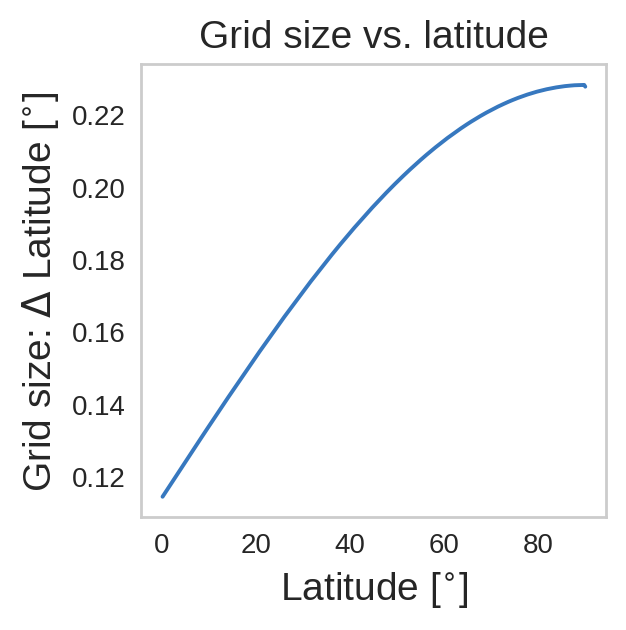
\includegraphics[width=\linewidth]{lat_diff_vs_lat.png}
\caption{Latitude was taken from IMS latitude file: rows 0 to 512, column 512, points plotted lie approximately at $80^{\circ}E$. Grid points are distributed densely near the equator, with latitude grid spacing of $.11^{\circ}$ at the equator. The latitude grid spacing increases to $.23^{\circ}$ at the north pole.}
\label{fig:lat_diff}
\end{minipage}
\end{figure}

This non-uniformity can be a source of confusion, leading to misinterpretations of the square kilometer estimation of snow coverage. This paper attempts to eliminate this confusion by explicitly calculating the surface area around each grid box of the $24 \times 24$ and $4 \times 4$ km resolution datasets.


IMS stores its data in zipped .asc files for each day. Each file includes header and a body. The body is in the form of a $n \times n$ matrix. The $24 \times 24$ km resolution has $n=1024$ and $4 \times 4$ km resolution has $n=6144$. Each point on the body is digits 0, 1, 2, 3, and 4 representing categorical information listed in Table 1. 

\begin{table}[hbt]
\centering
\caption{Meaning of the IMS categorical data.\label{tab1}}
{\begin{tabular}{|c|c|} 
\hline
\textbf{Data Marker} & \textbf{Meaning}
\\ \hline
0 & Out of the Earth surface range
\\ \hline
1 & Water
\\ \hline
2 & Land
\\ \hline
3 & Ice
\\ \hline
4 & Snow
\\ \hline
\end{tabular} }
\end{table}

The .asc files provided have two different formats; one described earlier and another deprecated format using 164 and 165 for ice and snow respectively. The latter format, occurring for years 1997 and 1998, does not include land and water values and uses irregular line breaks. TSM reformats the deprecated .asc files to include land and water digits and reshapes the data to match the standard $n \times n$ matrix format. 

For example, one .asc file displayed below shows only ice and snow (164 and 165), with irregular line breaks
\begin{verbatim}
   0    164    164    164    0    164    0    0    165    0    0    0  
   0    0      0      0      0    164    164  164  165    0    0    0  
\end{verbatim}
TSM later adds in land and sea values and converts the ice and snow values to 3 and 4, respectively. It also removes the irregular line breaks. The final data format is  shown below.
\begin{verbatim}
133313124222222223334000
\end{verbatim}
Under the new format, data for each day is in the an $n\times n$ matrix format, indexed by (row, column). The data matrix starts at (0,0) and ends at the point (n-1,n-1) See Fig.~\ref{fig:dry earth} for the $n\times n$ matrix coordinates.

Figure~\ref{fig:dry earth} is an illustration of the grid coordinate ticks on a stereographic projection square from NH without snow and ice information. The four black corner areas are marked as 0, which are out of the Earth surface range in the stereographic projection. The prime meridian in Fig.~\ref{fig:dry earth} is rotated clockwise by about 10.22$^{\circ}$. Additionally, the data is provided as a mirror image to what is shown in Figure~\ref{fig:dry earth}.
\begin{figure}[ht]
\centering
\begin{minipage}{4.0in}
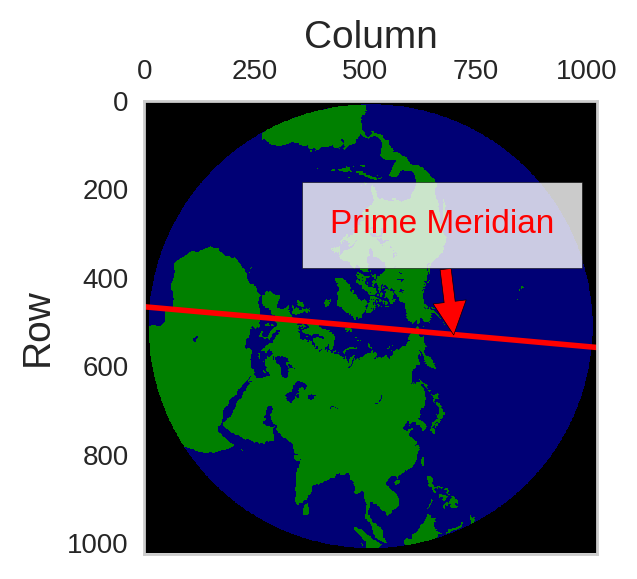
\includegraphics[width=\linewidth]{dry_planet_24km.png}
\caption{Grid coordinate ticks of NH without snow and ice cover. IMS provides daily files in an $n \times n$ format. The data is given in .asc files but mirrored to the figure shown. The file represents a stereographic projection, with the 80$^{\circ}$ meridian line pointing up. IMS rotates the prime meridian by about 10.22$^{\circ}$ clockwise to the horizontal. This figure shows the 24km resolution data, which has n = 1024.}
\label{fig:dry earth}
\end{minipage}
\end{figure}


Data is placed on a FTP server at \url{ftp://sidads.colorado.edu/pub/DATASETS/NOAA/G02156/}. FTP directory includes separate folders for lat-lon grids (metadata) and for each resolution. Data can be downloaded by selecting files in a directory while working in the browser. This process can be automated an FTP client/server software such as \gls{filezilla}. The dataset can be downloaded in parts or in its entirety and stored locally for manipulation. FileZilla can also syncronize local and remote directories. FTP server updates daily for each resolution folder.


Each IMS data file corresponds to one day. TSM main routine parses through each file and calculates the given area of snow and ice coverage. Python's Numpy, Pandas, and H5py libraries are used to handle daily datasets, grid area estimation, and database archives. TSM filters each file by the appropriate latitude and longitude and flattens it into a \gls{dataseries} object. TSM groups each series by year and stores them as a Hierarchal Data Format 5 (HDF5) file for each year. Basemap library is used for the projection transformations and plotting contours on maps.

TSM's main task calculates snow coverage for a given region. First, the .asc files are loaded into TSM, filtered to a region and then flattened into a vector, with each element is given a categorical index, notated by $T_k \in \{0,1,2,3,4\}$. $T_k$ is transformed into $B_k \in \{0, 1 \}$ where ice and snow values are transformed to 1 and everything else is transformed to 0. Each index has a corresponding area, computed by the shoe-lace formula and denoted by $A_k$.
The total area of snow and ice cover for a given day $t$ is simply the dot product between vectors $B_k$ and $A_k$:
\begin{equation}
Area_t  = B_k^{T}A_k
\end{equation}
Superscript $T$ is matrix transpose operator. The resulted data vector
$Area_t$ is added to an HDF5 database for each year.

$A_k$ is calculated by interpolating the latitude (lat) and longitude (lon) points, provided by NSIDC \cite{NIC}. The details are further explained later in this section. Latitude and longitude stored as binary .bin files and are loaded into TSM and formatted into $n \times n$ latitude and longitude matrices $\phi_{ij}, \lambda_{ij} \in {\rm I\!R}$, with i being the row of the .asc file and j the column.

Map projections showing snow and ice coverage from data files are generated using the Basemap library. TSM code has been placed in the public domain GitHub \cite{git_proj}. A blog about the TSM usage is posted on www.itsonlyamodel.us \cite{tibet_snow_man}.

TP region $25^{\circ}-45^{\circ}$N and $65^{\circ}-105^{\circ}$E is shown in Figure~\ref{fig:show_grid}. The grid box areas are shown by the contour plot in Figure~\ref{fig:show_grid} illustrate how the stereographic projection distorts the latitude spacing as latitude approaches the north pole, becoming coarser as latitude increases. Hence the area of a grid box varies according to latitude, as shown by the color contour in Figure~\ref{fig:areas_row_col}. One of TSM's main features is that it can calculate these grid areas.

\begin{figure}[ht]
\centering
\begin{minipage}{4.5in}
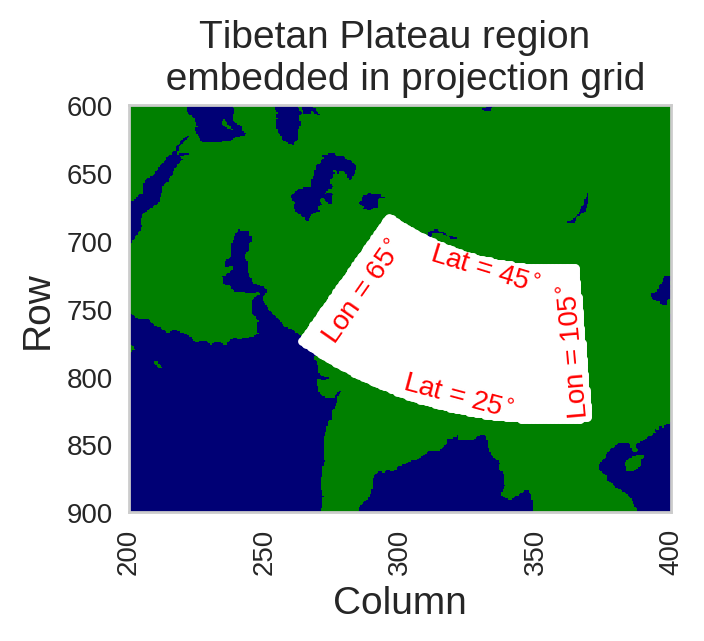
\includegraphics[width=\linewidth]{zoomed_earth.png}\\
\caption{The TP region ($25^{\circ}-45^{\circ}$N and $65^{\circ}-105^{\circ}$E) shown bounded in white is shown on a stereographic projection.}
\label{fig:show_grid}
\end{minipage}
\end{figure}

\begin{figure}[ht]
\centering
\begin{minipage}{6in}
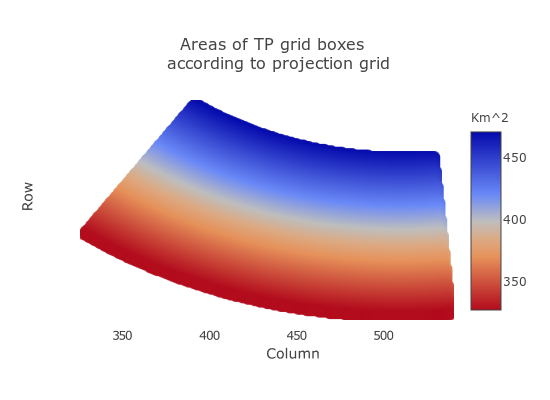
\includegraphics[width=\linewidth]{areas_of_tibet_grid_ii.png}
\caption{Color chart bottom shows grid box areas calculated using shoe-lace formula}
\label{fig:areas_row_col}
\end{minipage}
\end{figure}

Before calculating the area of a grid box, TSM estimates the box's corner points. Four points define a grid box, heron called centroids, because they are found by interpolating between four given lat-lon coordinates, (i,j), (i-1,j-1), (i,j-1), and (i-1,j). A zoomed in section showing this detail is provided for further clarification (see Figure~\ref{fig:areas_section} and \ref{fig:centroid_grid}). 
The surrounding four centroids $C_{i,j,k}$, indexed by $k=1,2,3,4$ for a given point $i,j$ are calculated as shown below.
\begin{align}
C_{ij1} &= \frac{1}{4}( p_{i-1,j-1}+ p_{i,j-1}+ p_{i,j} + p_{i-1,j} ) \\
C_{ij2} &= \frac{1}{4}( p_{i-1,j}+ p_{i-1,j+1} + p_{i,j+1}+ p_{i,j} ) \\
C_{ij3} &= \frac{1}{4}( p_{i,j}+ p_{i,j+1} + p_{i+1,j+1}+ p_{i+1,j} ) \\
C_{ij4} &= \frac{1}{4}( p_{i-1,j}+ p_{i,j} + p_{i+1,j} + p_{i-1,j+1} )
\end{align}
The area bounded four corners are calculated by first mapping them onto a 2d surface, and then by using the shoe-lace formula. See Figure~\ref{fig:centroid_grid} for reference.

\begin{figure}[ht]
\centering
\begin{minipage}{2.5in}
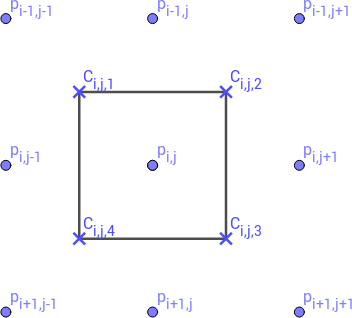
\includegraphics[width=\linewidth]{centroid_grid_w_box_cropped.png}
\caption{Grid box showing grid box corners $C_{i,j,k}$ for lat-lon point $p_{i,j}$ calculated using shoe-lace formula (\ref{eq:shoelace}).}
\label{fig:centroid_grid}
\end{minipage}
\end{figure}

The points are then projected onto a flat surface via the Lambert Azimuthal Equal Area Projection (LAEAP)\cite{snyder1987map}. LAEAP converts the lat-lon coordinates into Cartesian point x,y in meters about an arbitrary reference point $\phi_{1},\lambda_{0}$ using the following equations.

\begin{align}
x &= R k' \cos\phi_{1}\sin(\lambda - \lambda_0) \\
y &= R k'[\cos\phi_{1}\sin\phi - \sin\phi_{1}\cos\phi \cos(\lambda - \lambda_{0})] \\
k' &= \frac{\sqrt{2}}{\sqrt{1+\sin\phi_{1}\sin\phi + \cos\phi_{1}\cos\phi \cos(\lambda - \lambda_{0})}}
\end{align}
Where $R=6,371 km$ is the Earth's radius. For the TP, $\phi_{1} = 35^{\circ}$ $\lambda_{0}=85^{\circ}$ Treating these points as corners of a polygon, the areas are found using the discrete version of Green's Theorem, also known as the shoe-lace \cite{braden1986surveyor} formula shown below.
\begin{equation} \label{eq:shoelace}
A_{ij} = \frac{1}{2} \vert \sum\limits_{k=1}^{3}x_{k}y_{i+1} + x_{n}y_{1} - \sum\limits_{k=1}^{3}x_{k+1}y_{k} - x_{1}y_{n} \vert 
\end{equation}
where $A_{i,j}$ is area of point $i,j$, $k = 1,2,3$ represent the centroids that make up the corners of the polygon, $x_k$ and $y_k$ are vectors containing respective horizontal and vertical centroid coordinates. Once all the points were calculated, the ratio between largest and smallest grid area in Figure~\ref{fig:areas_tibet} was measured as $A_{ratio} = 1.44$.
\begin{figure}[ht]
\centering
\begin{minipage}{6in}
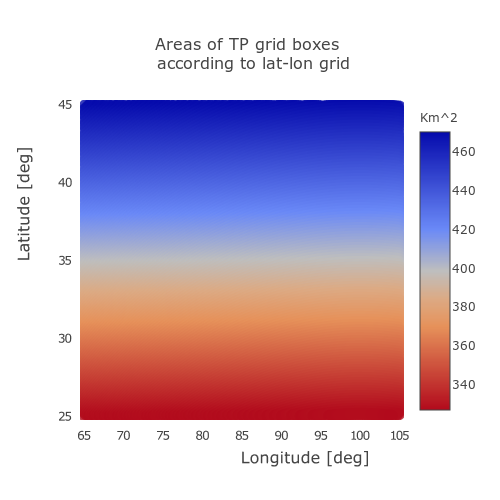
\includegraphics[width=\linewidth]{areas_of_tibet_grid_i.png}
\caption{The area of a grid box varies according to latitude.}
\label{fig:areas_tibet}
\end{minipage}
\end{figure}
To compare the areas gathered by the TSM project, an exact solution of the surface area of the TP region calculated by l'Huilier's formula for spherical triangles gives an area of 8,059,061.81 $km^2$. The $24 \times 24$ km area estimation made by Lambert equal area projection using the shoe-lace formula is 8,062,815.10 km (0.046 \% difference). The 4x4km area estimation is 8,061,716.81 $km^2$ (0.033 \% difference).

Zoomed in a small section, Figure~\ref{fig:areas_section} shows the four points surrounding each region.

\begin{figure}[ht]
\centering
\begin{minipage}{6in}
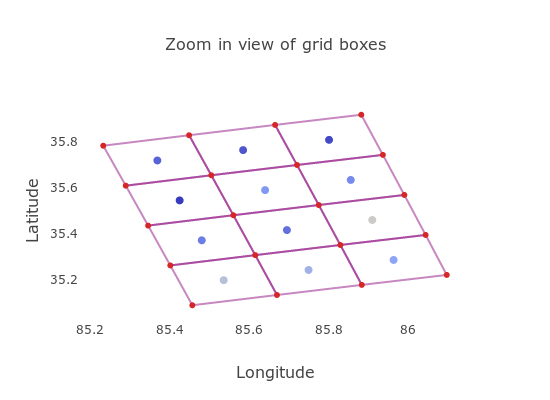
\includegraphics[width=\linewidth]{areas_of_subsection_i.png}
\caption{A zoom-in display of grid boxes and their centroid points provided a detailed view on how areas are estimated. Each central circle represents a lat-lon point provided by IMS. TSM calculates the red corner points followed by the bounding boxes' area.}
\label{fig:areas_section}
\end{minipage}
\end{figure}

IMS collects Snow data daily. The algorithm indicates snow and ice with a 1 and replaces land and sea with 0. That is, a given vector containing given values $T_k \in \{0,1,2,3,4\}$ is transformed to $B_k \in \{0,1\}$.

\begin{equation}
T_k \in \{0,1,2,3,4\} \mapsto B_k \in \{0,1\}
\end{equation}
The vector $B_k$ and the area vector $A_k$ is multiplied together by a dot product.
\begin{equation}
Area_t  = B_k^{T}A_k
\end{equation}
As an example, the top five points in Figure~\ref{fig:areas_section_ii} are covered in snow and are have $B_k$ values of 1. Shown in Figure~\ref{fig:areas_section}, the corners surrounding point i,k are calculated by taking the centroid of its surrounding four points.

\begin{figure}[ht]
\centering
\begin{minipage}{6in}
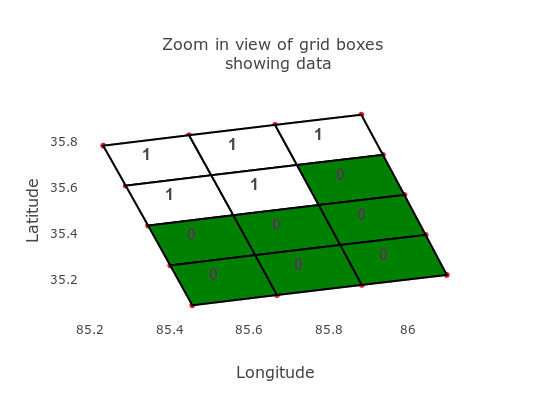
\includegraphics[width=\linewidth]{areas_of_subsection_ii.png}
\caption{A zoom-in view of the IMS data with snow/no snow illustrations. Cells covered in snow are in white and cells with no snow are shown in green.}
\label{fig:areas_section_ii}
\end{minipage}
\end{figure}


The Earth is modeled as a sphere of radius $R = 6,371 \ km$ The Haversine function calculates the great circle distance between two lat-lon points in degrees.

\begin{eqnarray}
\Delta \phi &=& \phi_{2} - \phi_{1} \\
\Delta \lambda &=& \lambda_2- \lambda_1 \\
a &=& \sin(\frac{\Delta \phi}{2})^{2} + \cos(\phi_1)  \cos(\phi_2)  \sin(\frac{\Delta \lambda}{2})^{2} \\
c &=& 2  \arcsin(\sqrt(a))
\end{eqnarray}
where $\phi$ represents latitude and $\lambda$ represents longitude and c is the great circle length in degrees.
Next, a semi perimeter area is calculated
\begin{equation}
s = c + \pi + \frac{\phi_{1} + \phi_{2}}{2}
\end{equation}
Finally, The area of a spherical triangle is given by the l'Huilier formula
\begin{eqnarray}
b &=& \left(
\tan(\frac{s}{2})
\tan(\frac{s-d}{2})
\tan(\frac{s - \pi/2 + \phi_{1}}{2})
\tan(\frac{s - \pi/2 + \phi_{2}}{2}) \right)^{\frac{1}{2}} \\
\Delta &=& 4.0 * \arctan(b)
\end{eqnarray}
where $\Delta$ is the radial area of a spherical triangle. 

Treating the longitude points $\lambda_1 = 65^{\circ}$ $\lambda_2 = 105^{\circ}$ and setting $\phi_{1} = \phi_{2}$. Two different spherical triangle areas are obtained for $\phi_{top} = 45^{\circ}$ $\phi_{bottom} = 25^{\circ}$, $\Delta_{top}$ and $\Delta_{bottom}$ are obtained. The area of Tibet in $km^2$ is given by 
\begin{equation}
A_{tibet} = R^2(\Delta_{top} - \Delta_{bottom}),
\end{equation}
where $A_{tibet}$ is treated as the exact solution and compared to the sum of areas in our data frame


Snow data are visualized by plotting an interpolated contour grid onto a Mercator projection of the TP, region shown in Figure~\ref{compare_grids}.
\begin{figure}[ht]
\centering
\begin{minipage}{6in}
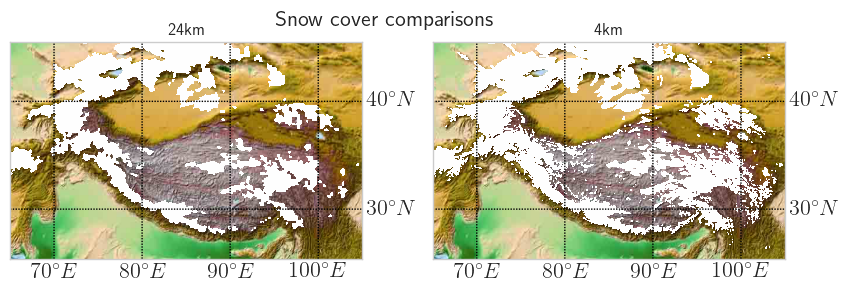
\includegraphics[width=\linewidth]{tibet-snow-res-compare.png}
\caption{Tibetan plateau region's snow cover for 2 January 2015: The white region indicates snow cover which is over layed on the land surface topography.}
\label{compare_grids}
\end{minipage}
\end{figure}
The two grids are compared in a time series of snow coverage collected from 2004-02-24 until 2017-06-26, shown in Fig. ~\ref{compare_times_series}. A percent coverage difference subplot is included to better distinguish between the two series,defined as:

\begin{equation}\label{eq:perc_diff}
100 * \left( \frac{ts_{24\ km} - ts_{4\ km}}{ts_{4\ km}} \right),
\end{equation}
where $A_{tibet}= 8,059,061.82 km^{2}$ Calculated analytically via the l'Huilier's formula for spherical triangles.

Figure~\ref{compare_times_series} indicates a percent coverage difference range of $[-10.12 \%, 48.42 \%]$. Note The finer resolution grid reports more snow coverage in the warmer months, suggesting the finer grid records glaciers and smaller snowfields. During winter and spring months, this trend reverses, with the finer resolution grid reporting less snow and ice coverage, indicating a positive bias for the 24x24 km resolution product. 

\begin{figure}[ht]
\centering
\begin{minipage}{6in}
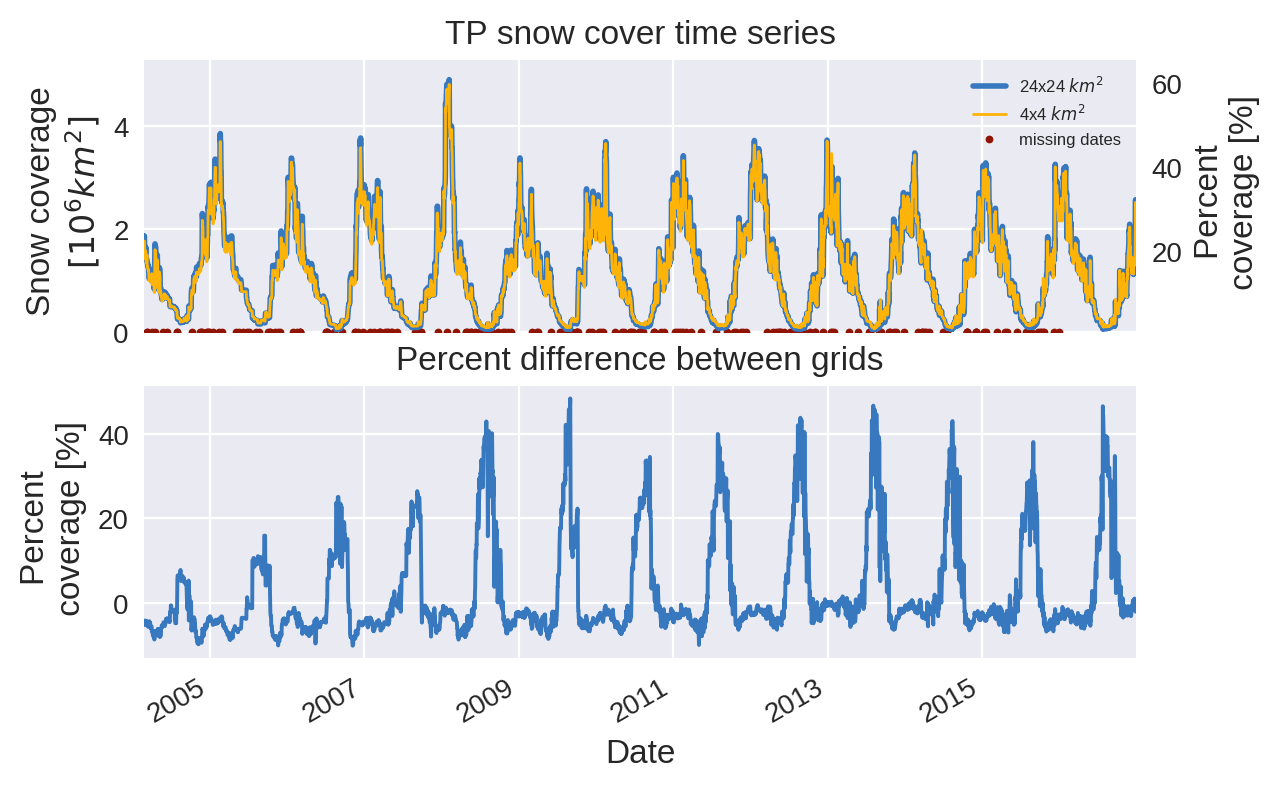
\includegraphics[width=\linewidth]{ts-2-res.png}
\caption{The snow cover area time series comparison between two resolutions: 4 km and 24 km. Percent difference calculated using (~\ref{eq:perc_diff}).}
\label{compare_times_series}
\end{minipage}
\end{figure}
%TODO: verify end date
Figure~\ref{compare_area_methods} shows a time series showing percent coverage collected until from 1997-02-04 until 2017-06-26. An area estimation conducted by Shen et al. \cite{shen2015TPSC} assumed a uniform $24x24 km^{2}$ grid area. This assumption causes an overestimation of snow and ice coverage by as little as 32.2 \% and as much as 54.79 \%.

\begin{figure}[ht]
\centering
\begin{minipage}{6in}
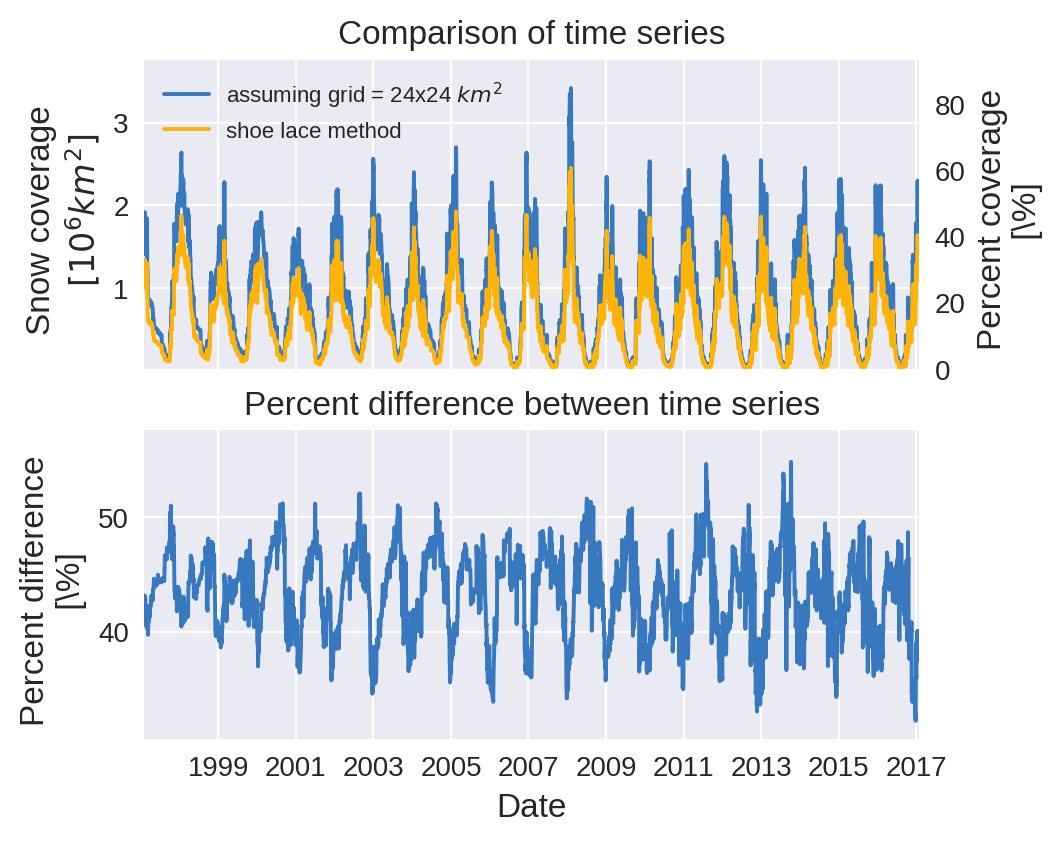
\includegraphics[width=\linewidth]{ts-compare.png}
\caption{Time series comparison between $24\times 24 km^{2}$ assumption and area calculation via shoe-lace formula.}
\label{compare_area_methods}
\end{minipage}
\end{figure}

Long-term trends in snow cover are obtained by binning the annual cycles into 5 day periods and averaging them, denoted by $clim(t)_{5}$. The annual snow cycle is shown in Figure~\ref{fig:clim} This annual snowfall is subtracted from the time series, $Snow(t)$.
\begin{equation}
Anomalies(t) = Snow(t)-clim(t)_{5}
\end{equation}
From there a linear regression is obtained that is not influenced by annual cycle, shown in Fig.~\ref{anomalies}

\begin{figure}[ht]
\centering
\begin{minipage}{6in}
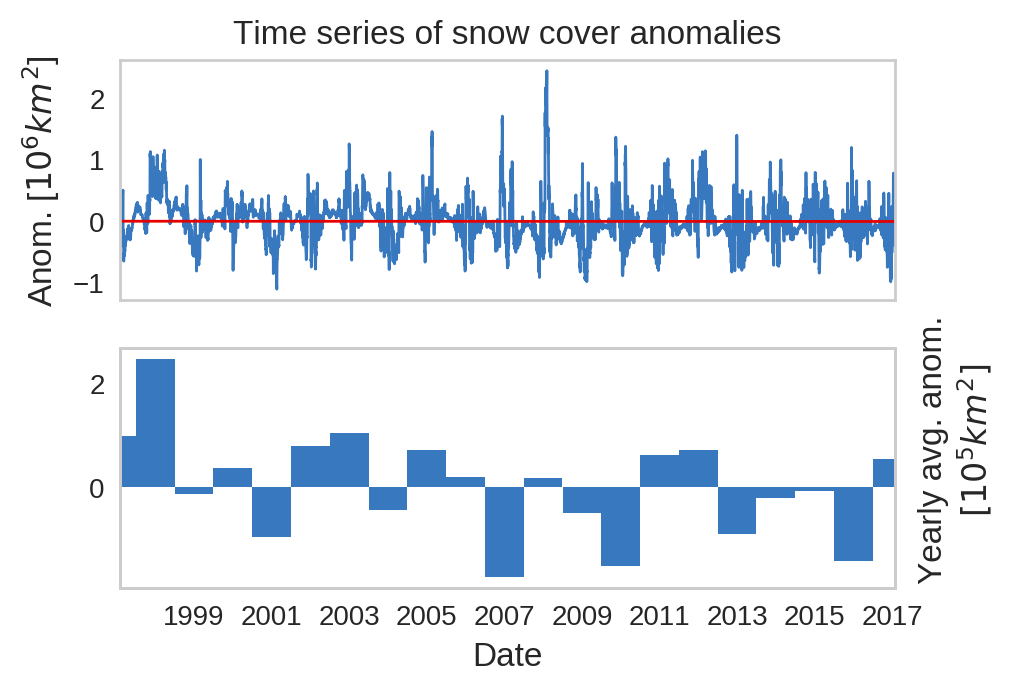
\includegraphics[width=\linewidth]{tibet-24-anomalies-ts.png}
\caption{Time series of Snow coverage anomalies with included trend line, in addition to yearly averaged anomalies, shown by the bar chart.}
\label{anomalies}
\end{minipage}
\end{figure}

A trend line was included to investigate long-term trends on the plateau. Linear regression results indicate no significant trends in snow coverage from the start of the IMS product to the last date of capture. There is little indication of a considerable change in snow coverage with the data provided; though, there is a high certainty of a negative change. Still, the yearly averaged anomaly bar chart show greater frequencies of yearly averaged negative anomalies in recent years, suggesting there is some change taking place in the TP snowpack.

Climate averaging $clim(t)_{5}$ shown in Figure~\ref{fig:clim} provides an expected annual snow coverage profile for the TP. Maximum snow coverage at $2.786 \ 10^{6} km^{2}$ occurs in January 21th till January 25th. Minimum snow coverage at $0.151 \ 10^{6} km^{2}$ occurs from August 24th till August 28th. Annual mean coverage = 1.199x$10^6\ km^2$

\begin{figure}[ht]
\centering
\begin{minipage}{3in}
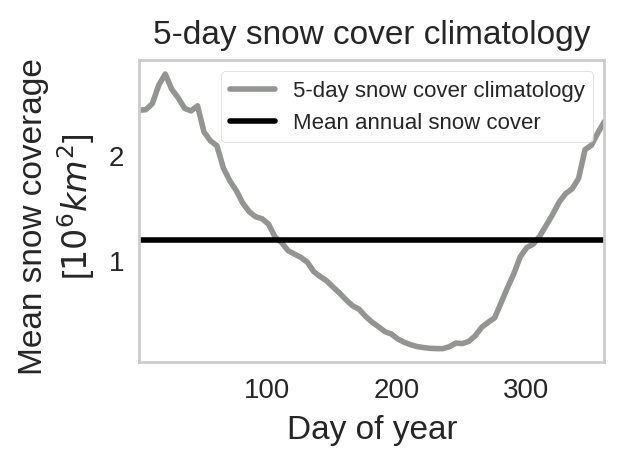
\includegraphics[width=\linewidth]{tibet-24-climate.png}
\caption{5 day climate averages of the $24 \times 24$ km annual snow cycle.}
\label{fig:clim}
\end{minipage}
\end{figure}

Figure~\ref{fig:hist} is a histogram showing the probabilistic distribution. Kurtosis is given using Pearson's definition. \cite{kokoska2000standard}

\begin{figure}[ht]
\centering
\begin{minipage}{3in}
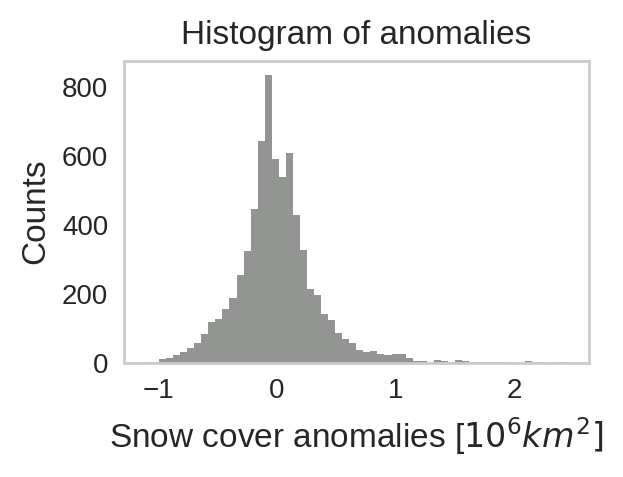
\includegraphics[width=\linewidth]{tibet-24-anomalies-hist.png}
\caption{Histogram of the $24 \times 24$ anomalies.}
\label{fig:hist}
\end{minipage}
\end{figure}

\begin{table}[hbt]
\centering
\caption{Anomaly Distribution Properties \label{anom_table}}
{\begin{tabular}{|c|c|}
\hline
\textbf{Statistic} & \textbf{Value}
\\ \hline
Mean\hphantom{00} & \hphantom{0}$-309.9 km^{2}$
\\ \hline
Median\hphantom{00} & \hphantom{0}$-30992 km^{2}$
\\ \hline
Min\hphantom{00} & \hphantom{0}$-1.112\ 10^6 km^{2}$
\\ \hline
Max\hphantom{00} & \hphantom{0}$2.446\ 10^6 km^{2}$
\\ \hline
Standard Deviation\hphantom{00} & \hphantom{0}$.34259971\ 10^6 km^{2}$
\\ \hline
Skew\hphantom{00} & $1.0006$
\\ \hline
Kurtosis (Pearson's) \hphantom{00} & $4.351$
\\ \hline
\end{tabular} }
\end{table}

Maximum snow coverage was reported on 2008-02-06, during one of most volitle weather patterns in China's recent history \cite{bbc}. The surge in 2008 winter storms are thought to be caused by a combination of La Nina and cold temperatures \cite{reutersUK}.

Minimum snow coverage was reported on 2013-08-12, which was known for its unusually warmer weather in Southern China\cite{NOAANCDC}.

The standard deviation is approximately a quarter of the annual mean. Such a large standard deviation implies a high risk of snowstorms and the general volatility of water sources coming from the TP.   

Both Skew and Kurtosis tests gave p-values of approximately zero.

Skew greater than 1 indicates more outliers to the right of the mean, suggesting that the TP experiences severe snow storms, compared to a steady flux of predictable snow patterns. 

Kurtosis is greater than three shows that anomalies gather closer to the mean when compared to a Gaussian distribution. The expected snow cover occurs often, but infrequent storms can create large anomalies.

Climate averaged anomalies allow basic statistics. However there are some drawbacks, chiefly, the long-term trends and noise remain coupled. An alternative approach to anomalies, seasonal decomposition by LOESS can attempt breaking a time series into three components: season, trend, and remainder. This non-parametric method is described in the Appendix\ref{append:STL}. The results shown in Figure~\ref{fig:24_stl} reveals a remainder that appears to be almost identical to the five days averaged climate anomalies from Figure~\ref{anomalies}. The trend portion does not appear to have a clear increase or decrease. Large peaks occur on winter months 1998 and 2017 which is also seen in the yearly averaged anomalies.

\begin{figure}[ht]
\centering
\begin{minipage}{3in}
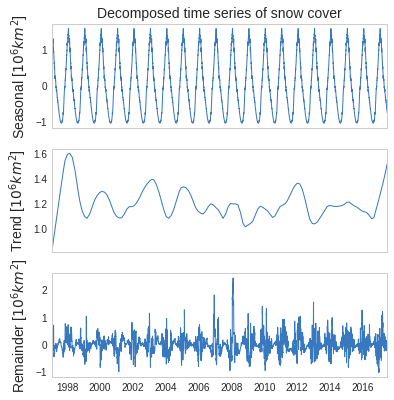
\includegraphics[width=\linewidth]{tibet-24-stl.png}
\caption{Deseasonalized using STL algorithm described in Appendix.}
\label{fig:24_stl}
\end{minipage}
\end{figure}

Another advantage to using seasonal decomposition by LOESS is that it will fill in missing values with approximations, creating a daily time series with no missing values. By removing the seasonal portion, the remainder and trend can be modeled as a stationary linear time series. Details on the theory are explained in Appendix \ref{append:TS}. The series' variance is seasonal. Therefore the time series log transform is taken. An AR(6) model is selected to have the more favorable AIC while still passing the Box-Ljung test.

\begin{equation}
log(Z_t) = a_{t} + \theta_1 a_{t-1} + \theta_2 a_{t-2} + \theta_3 a_{t-3} + \theta_4 a_{t-4} + \theta_5 a_{t-5} + \theta_6 a_{t-6}
\end{equation}

\begin{table}[hbt]
\centering
\caption{AR(6) model parameters with AIC = -12046.12 \label{tbl:ar6}}
{\begin{tabular}{|c|c|c|}
\hline
\textbf{Param} & \textbf{Value} & \textbf{Standard Error}
\\ \hline
$\theta_1$ & 1.0099 & 0.0116
\\ \hline
$\theta_2$ & -0.0814 & 0.0165
\\ \hline
$\theta_3$ & -0.0395 & 0.0165
\\ \hline
$\theta_4$ & 0.0460 & 0.0165
\\ \hline
$\theta_5$ & -0.0234 & 0.0165
\\ \hline
$\theta_6$ & 0.0214 & 0.0116
\\ \hline
intercept & 13.9548 & 0.0186
\\ \hline
$\sigma^2$ & 0.01159 & N/A \\ \hline
\end{tabular}}
\end{table}

The AR(6) model with estimated parameters shown in Table~\ref{tbl:ar6} have a relatively low AIC = -12046.12 and a Box-Ljung test that fails to reject the null hypothesis, shown in Figure~\ref{fig:BL}. All of the calculated, $p-values>.005$ indicating that the residuals after fitting the AR(6) model to the deseasonalized snow data are not autocorrelated.

\begin{figure}[ht]
\centering
\begin{minipage}{3in}
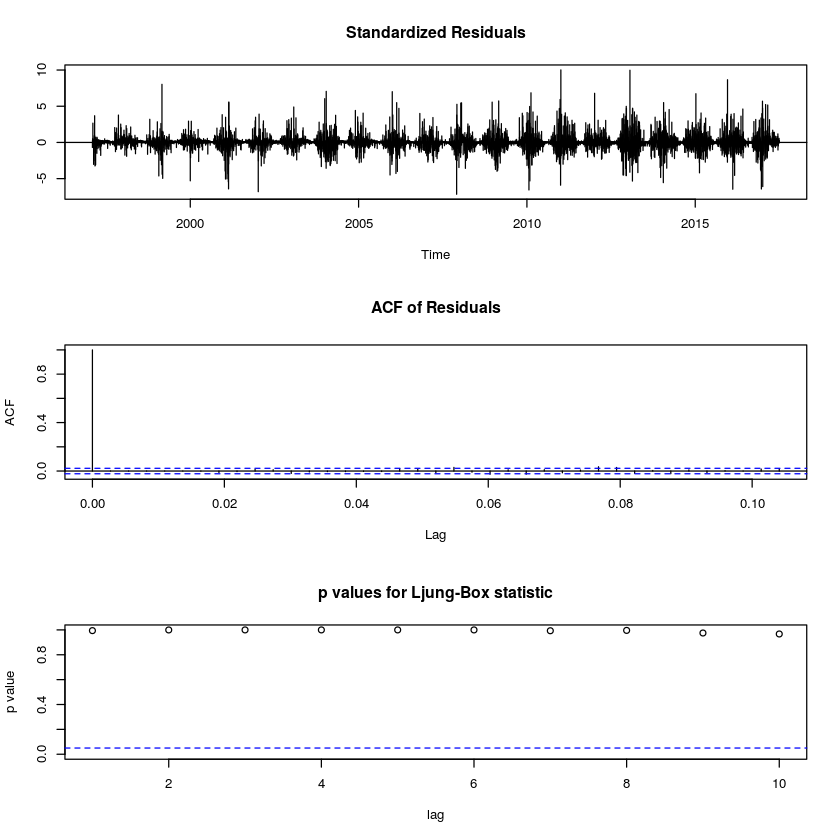
\includegraphics[width=\linewidth]{BL.png}
\caption{Box-Ljung diagnostic test for $m=10$ of an AR(6) model. For all lags, $p-values>.005$ indicating that the residuals after fitting the AR(6) model are not autocorrelated.}
\label{fig:BL}
\end{minipage}
\end{figure}


The TSM is currently used to generate daily snow mapping at \url{http://www.itsonlyamodel.us/daily-snow.html}. See Figure~\ref{fig:daily_map}.

\begin{figure}[ht]
\centering
\begin{minipage}{4in}
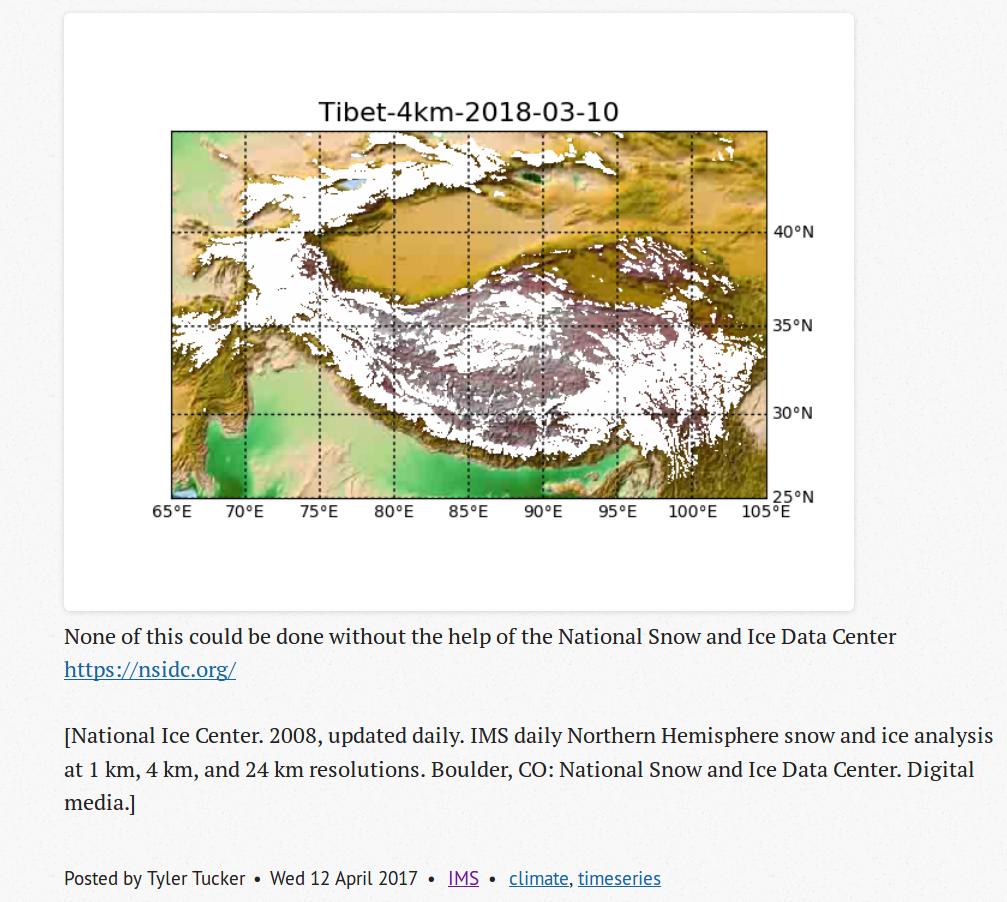
\includegraphics[width=\linewidth]{daily-tsm.png}
\caption{Screenshot of daily snow plot at \url{http://www.itsonlyamodel.us/daily-snow.html}}
\label{fig:daily_map}
\end{minipage}
\end{figure}

The Chinese National Earth System Science Data Sharing Infrastructure website uses TSM to archive current and past snow coverage of TP at \url{http://www.tpedatabase.cn/tibetSnow.jsp}\cite{TP_database} shown by Figure~\ref{fig:ch_daily_map}. As of now, the tool is primarily used for generating images; however, we have shown that the TSM can be used for analysis.

\begin{figure}[ht]
\centering
\begin{minipage}{4in}
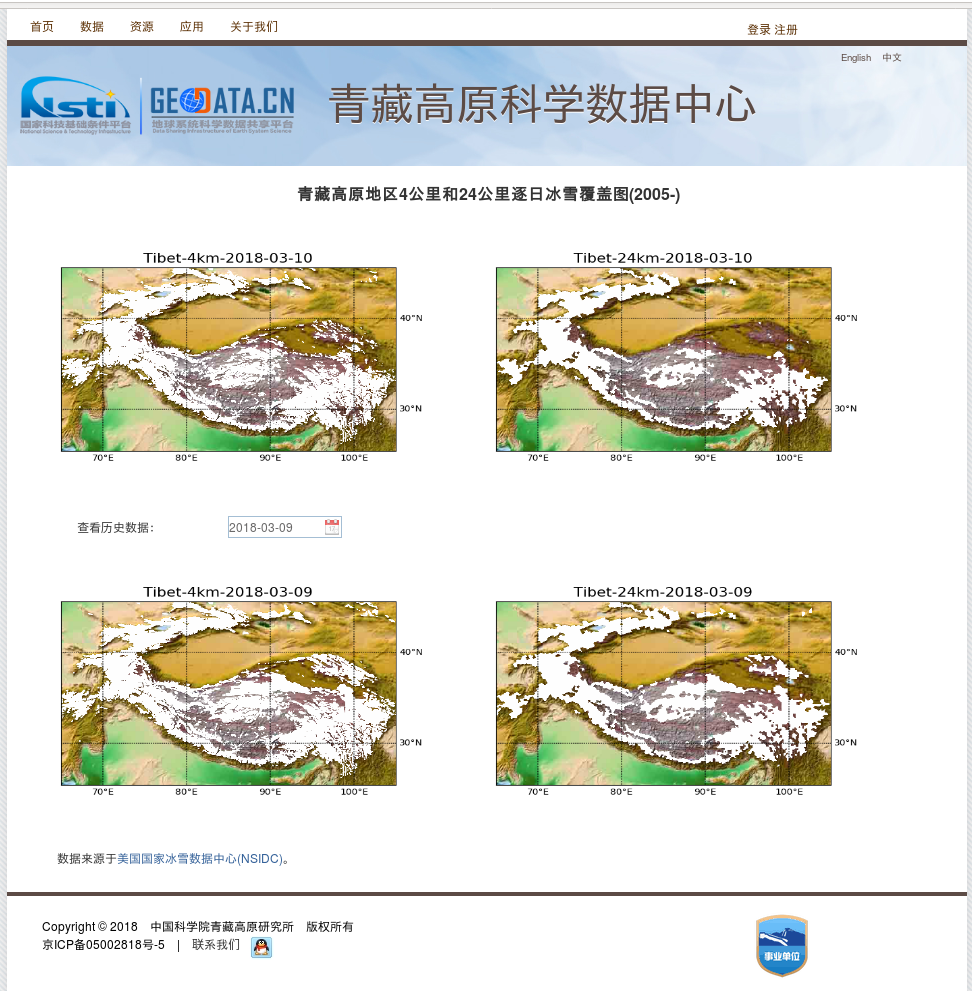
\includegraphics[width=\linewidth]{tpe-daily.png}
\caption{Screenshot of \url{http://www.tpedatabase.cn/tibetSnow.jsp} showing daily snow plot at archives at 24 and 4 km resolution.}
\label{fig:ch_daily_map}
\end{minipage}
\end{figure}


The TSM project provided on GitHub \cite{git_proj} is a convenient tool for parsing through large IMS data sets. Statistical inferencing using this set has never been easier or more accessible to both professional and amateur alike. Anyone who can run a python environment can generate time series, snow and ice maps, histograms, spectral series over TP or any region over the Northern Hemisphere. TSM provides users with data sets that can be used for statistical inferencing as shown by the simple statistical inferencing in the results section.

Regression trends point out less snow over the TP today than at the onset of the IMS project. Histogram trends outline that it is more likely for there to be negative anomalies than positive ones.

Analysis can be made using either the fine or coarse data set. The project created offers researchers a toolkit that quickly parses through massive data sets over any latitude and longitude range in the northern hemisphere. 

TSM can adjust the map projection reference location, in the case that IMS begins recording snow and ice coverage over the Southern Hemisphere.

Moreover, calculated areas improve the accuracy of these gridded measurements, and aid in monitoring snow and ice data sets. 

Future developments to TSM can include better means of querying subsets of data. Current methods do not use a database but depend on local files. A database with a website interface would give more users access to more data. The scalability of the dataset also makes it possible to implement the 1x1 km data set. The higher resolution set could show the change in glacier and ice field size over time and even pinpoint regions of rapid climate change. A database design also can be continually updated with the NSIDC's daily measurements. Lastly, a website interface would give users with no python experience access TSM. The next chapter describes this web-app framework used by the ARGO project. A similar web app can be created for IMS, providing a much-needed service for SACD for this and related products.